\chapter{Qualità nelle modulazioni analogiche}

\begin{figure}[h]
    \centering
    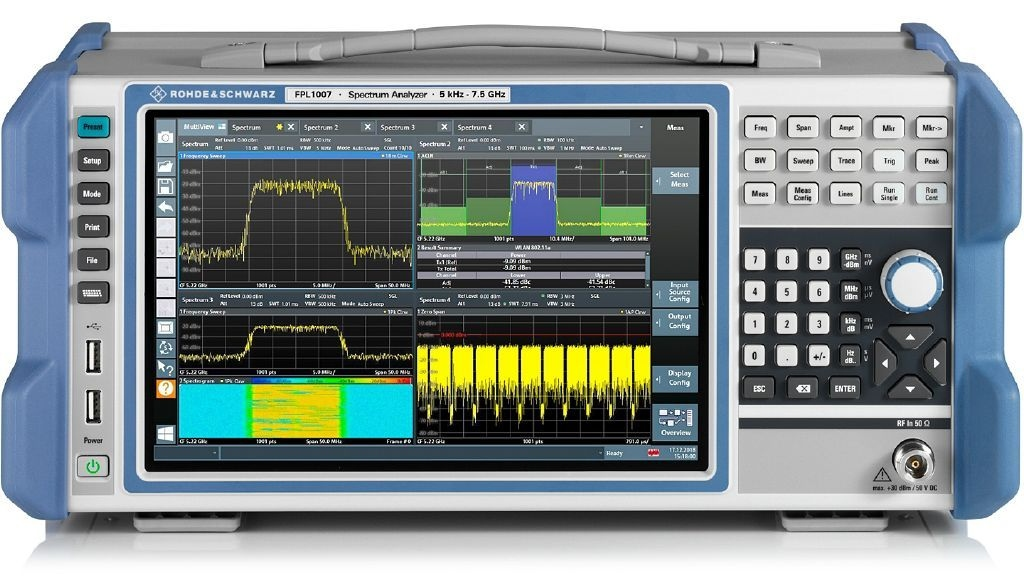
\includegraphics[scale = 0.3]{fpl1000-spectrum-analyzer-front.jpg}
\end{figure}

\newpage 

\section{Sistema in banda base}
\footnote{Slide del prof | Qualità nelle modulazioni analogiche | pag 1.1 \\  
Appunti di Damiano| pag 1.1 \\
Slide | Qualità nelle modulazioni analogiche | pag 1.1 \\
Appunti | 2025-03-10 | pag 5 - 6 \\ 
Appunti | 2025-07-08 Ricevimento | pag 8.2} 

\begin{tcolorbox}
    Stai molto attento alla terminologia utilizzata in questo capitolo perché può differire dagli altri capitoli, 
    quindi prima leggi sopra la descrizione e la spiegazione della formula, poi applicala al compito scritto / negli esercizi
\end{tcolorbox}

Consideriamo, al momento, solo il sistema in banda base. \newline 

Il ricevitore è costituito da un filtro passa-basso con banda W, dove W è la larghezza di banda del segnale utile. \newline 

Se il filtro passa-basso ha una banda W minore della banda del segnale ricevuto, 
il segnale ricevuto verrà distorto. \newline 

Se il filtro passa-basso ha una banda W maggiore della banda del segnale ricevuto, 
il segnale ricevuto non verrà distorto, ma il filtro aggiungerà del rumore sulle frequenze aggiunte. \newline 

\begin{tcolorbox}
    Considera la banda del filtro passa-basso come l'altezza di una porta. \newline 

    Se io sono una persona molta alta (segnale ricevuto a banda larga) ed ho una porta molto alta, 
    posso tranquillamente entrare nella stanza (segnale ricevuto non distorto) rimanendo intatto, ma avrai dei tacchi in modo da avere la stessa altezza della porta (aggiunta del rumore). \newline 

    Se io sono una persona molto alta ed ho una porta molto bassa, o non ci passo o dovrei "tagliarmi" in più pezzettini (segnale ricevuto distorto).
\end{tcolorbox}

In formule, il $\left( \frac{S}{N} \right)_{b}$ è: 

{
    \Large 
    \begin{equation}
        \left( \frac{S}{N} \right)_{b}
        = 
        \frac{P_R}{N_0 \cdot W}
    \end{equation}
}

dove: 

\begin{itemize}
    \item $\left( \frac{S}{N} \right)_{b}$ è il rapporto segnale rumore in banda base (dall'inglese base-band Signal-to-Noise ratio) 
    \item $P_r$ è la potenza utile ricevuto 
    \item $P_{n_o}$ è la potenza di rumore termico in uscita
\end{itemize}

Come abbiamo studiato nei precedenti capitoli, 
la potenza di rumore termico in uscita da un filtro vale ideale: 

{
    \Large 
    \begin{equation}
        \begin{split}
        P_{n_o}
        &= 
        \int_{-W}^{+W} 
        \frac{N_0}{2}
        df
        \\
        &= 
        N_0 \cdot W
        \end{split}
    \end{equation}
}

dove $\frac{N_0}{2}$ è la densità spettrale di rumore termico bilatera in ingresso. \newline 

Il nostro obbiettivo è quello di esprimere il rapporto segnale rumore per le varie tecniche di modulazione, 
in termini del rapporto segnale-rumore in banda base. \newline 

In formule: 

{
    \Large 
    \begin{equation}
       \left( \frac{S}{N} \right)_{o}
       = 
       A \cdot \left( \frac{S}{N} \right)_{b} 
    \end{equation}
}

dove: 

\begin{itemize}
    \item $\left( \frac{S}{N} \right)_{o}$ è il rapporto segnale rumore dopo la modulazione 
    \item $\left( \frac{S}{N} \right)_{b} $ è il rapporto segnale rumore in banda base 
    \item A è un coefficiente moltiplicativo di qualità della modulazione
\end{itemize}

Il coefficiente moltiplicativo A della qualità della modulazione può assumere diversi valori. \newline 

Se $A = 1$, la modulazione ha la stessa qualità del segnale in banda base, cioè: 

{
    \Large 
    \begin{equation}
       \left( \frac{S}{N} \right)_{o}
       = 
        \left( \frac{S}{N} \right)_{b} 
    \end{equation}
}

Se $A < 1$, la modulazione ha una prestazione inferiore rispetto al segnale in banda base, cioè: 

{
    \Large 
    \begin{equation}
        \left( \frac{S}{N} \right)_{o}
       < 
        \left( \frac{S}{N} \right)_{b} 
    \end{equation}
}

Se $A > 1$, la modulazione ha una prestazione migliore rispetto al segnale in banda base, cioè: 

{
    \Large 
    \begin{equation}
        \left( \frac{S}{N} \right)_{o}
       > 
    \left( \frac{S}{N} \right)_{b} 
    \end{equation}
}

\begin{tcolorbox}
    Come vedremo in seguito, alcune modulazione avranno un SNR peggiore in modulazione rispetto all'SNR in banda base, 
    ma verranno scelte quelle modulazioni non per la qualità ma per altri pregi. \newline 

    Ad esempio l'AM-convenzionale avrà un SNR peggiore in modulazione rispetto all'SNR in banda base, 
    ma verrà scelta perché il demodulatore ha un basso costo economico di progettazione. 
\end{tcolorbox}

Quando si fa un progetto, generalmente si fissa l'SNR e poi si realizza il progetto. \newline 

\begin{tcolorbox}
Il progettista del sistema di telecomunicazioni fissa un SNR in banda base che deve essere in uscita dal ricevitore. \newline 

Lo stadio in cui si analizza e quantifica il rapporto segnale-rumore in banda base dipende dal progetto. \newline 

Il termine ricevitore, generalmente (ma può variare a caso a caso) 
si intende a valle, cioè in uscita, del ricevitore, in particolare lo stadio dopo la demodulazione. \newline 

Ad esempio, se ci troviamo in radio-frequenza, possiamo fissare e progettare l'SNR in banda base
dopo lo stadio di ingresso del ricevitore (cioè il segnale dopo l'antenna, dopo il cavo dall'antenna alla radio, dopo la radio al demodulatore). \newline 

Ma in altri casi lo si può fissare dopo il quantizzatore. \newline 

Come tutti gli episodi della vita, dipende. \newline 

\url{https://www.youtube.com/watch?v=cf_ITVX7qCg} \\
JARABE DE PALO - "DIPENDE" (Video Oficial en italiano)
\end{tcolorbox}

\newpage 


\section{Qualità della DSB-SC}
\footnote{Slide del prof | Qualità nelle modulazioni analogiche | pag 1.2 - 3.1\\  
Appunti di Damiano| pag 1.2 - 3.1 \\
Slide | Qualità nelle modulazioni analogiche | pag 1.2 - 3.1 \\
Appunti | 2025-03-10 | pag 6 - 8} 

Focalizziamoci adesso sulla DSB-SC. \newline 

Dai capitoli precedenti, sappiamo che il segnale modulato in DSB-SC u(t) ha la seguente formula (considerando $\phi_c = 0$ per semplicità di notazione): 

{
    \Large 
    \begin{equation}
        \begin{split}
            u (t) 
            &= 
            m(t) \cdot c(t)
            \\
            &=
            m(t) \cdot \left[ A_c \cdot \cos(2 \pi f_c t + \phi_c) \right]
            \\
            &= 
            \left[A_c \cdot m(t) \right] \cdot \cos(2 \pi f_c t + \phi_c)
            \\
            &= 
            A_c m(t) \cos(2 \pi f_c t + \phi_c)
            \\
            &\downarrow 
            \\
            u(t)
            &=
            A_c m(t) \cos(2 \pi f_c t + 0)
            \\
            &=
            A_c m(t) \cos(2 \pi f_c t)
        \end{split}
    \end{equation}
}

dove: 

\begin{itemize}
    \item u(t) è il segnale modulato in DSB-SC 
    \item m(t) è il segnale modulante 
    \item c(t) è il segnale della portante
\end{itemize}

Considerando un rumore additivo n(t) perché è AWGN, 
allora il segnale che riceviamo r(t) è uguale a: 

{
    \Large 
    \begin{equation}
        \begin{split}
            r(t) 
            &= 
            u(t) + n(t)
            \\
            &=
            \left[
                A_c m(t) \cos(2 \pi f_c t)
            \right]
            +
            \left[
                n_c (t) \cos(2 \pi f_c t)
                - 
                n_s(t) \sin(2 \pi f_c t)
            \right]
        \end{split}
    \end{equation}
}

dove: 

\begin{itemize}
    \item $n_c (t)$ è la componente del rumore in fase 
    \item $n_s (t)$ è la componente di rumore in quadratura
\end{itemize}

\newpage 

Utilizzando il piano dei fasori, 
possiamo visualizzare n(t): 

{
    \Large 
    \begin{equation}
        n(t)
        =
        n_c (t) \cos(2 \pi f_c t)
        - 
        n_s(t) \sin(2 \pi f_c t)
    \end{equation}
}

come: 

\begin{figure}[h]
    \centering
    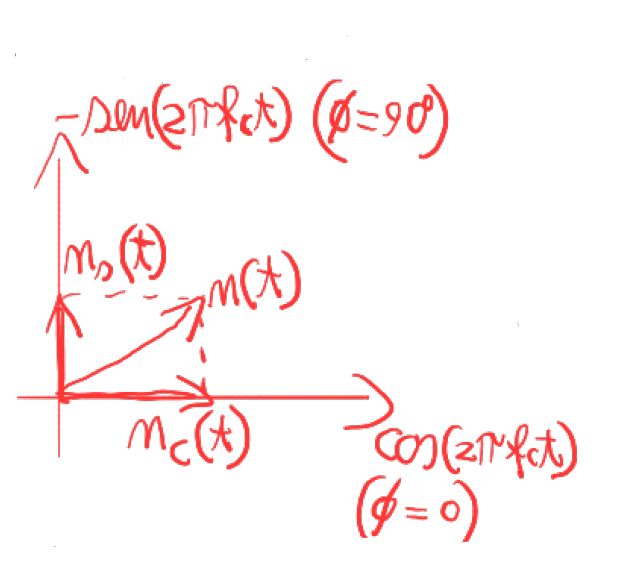
\includegraphics[scale = 0.8]{Proiezione del rumore nel piano fasoriale.PNG}
\end{figure}

Quindi il rumore n(t) è un vettore, in cui $n_c (t)$ è la proiezione di n(t) dell'asse dei coseni, 
$n_s (t)$ è la proiezione del rumore n(t) nell'asse dei seni. \newline 

Ma, dalla teoria dei Segnali Determinati Aleatori, sappiamo che: 

{
    \Large 
    \begin{equation}
        < n_c (t) > \text{ }
        =
        \text{ }
        < n_c (t) > 
        \text{ }
        = 
        \text{ }
        0
    \end{equation}
}

essendo un rumore AWGN, il valore medio del rumore n(t) è nullo. \newline 

Invece, per quanto riguarda la varianza del rumore n(t): 


{
    \Large 
    \begin{equation}
        < n_c ^{2} (t) > \text{ }
        =
        \text{ }
        < n_c ^{2} (t) > 
        \text{ }
        = 
        \text{ }
        < n ^{2} (t) > 
        \text{ }
        = 
        \text{ }
        \sigma_n ^{2}
    \end{equation}
}

cioè, in parole e per esteso, il valore medio quadratico del rumore $< n ^{2} (t) > $ è uguale alla varianza del rumore $\sigma_n ^{2}$. \newline 

Per la demodulazione, scegliamo un demodulatore coerente, ciò significa moltiplicare r(t) per un coseno con la frequenza $f_c$ della portante. \newline  

In formule step-by-step, se consideriamo y(t) il segnale demodulato in modo coerente: 

{
    \Large 
    \begin{equation}
        \begin{split}
            y(t)
            &= 
            r(t) \cdot \cos(2 \pi f_c t)
            \\
            &= 
            A_c m(t) \cos[2](2 \pi f_c t)
            +
            n_c(t) \cos[2](2 \pi f_c t)
            -
            n_s(t) \sin(2 \pi f_c t) \cos(2 \pi f_c t)
            \\
            &=
            \frac{A_c m(t)}{2}
            + 
            \frac{A_c m(t) \cos(4 \pi f_c t)}{2}
            +
            \frac{n_c (t)}{2}
            +
            \frac{n_c (t) \cos(4 \pi f_c t)}{2}
            - 
            \frac{n_s (t) \sin(4 \pi f_c t)}{2}
        \end{split}
    \end{equation}
}

\newpage 

Ricordando lo schema di una demodulazione coerente: 

\begin{figure}[h]
    \centering
    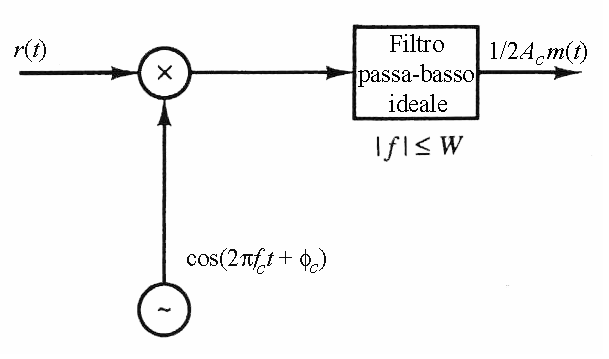
\includegraphics[scale = 1]{Schema architettura di un demodulatore.png}
\end{figure} 

togliamo dal segnale demodulato tutte le componenti oltre a $2 \pi f_c t$, 
che fisicamente verranno tolte dal filtro passa-basso ideale: 

{
    \Large 
    \begin{equation}
        \begin{split}
            y(t) 
            &=
            \frac{A_c m(t)}{2}
            + 
            \frac{A_c m(t) \cos(4 \pi f_c t)}{2}
            +
            \frac{n_c (t)}{2}
            +
            \frac{n_c (t) \cos(4 \pi f_c t)}{2}
            - 
            \frac{n_s (t) \sin(4 \pi f_c t)}{2}
            \\
            &\downarrow
            \\
            y(t)
            &=
            \frac{A_c m(t)}{2}
            + 
            0
            +
            \frac{n_c (t)}{2}
            +
            0
            - 
            0
            \\
            &= 
            \frac{A_c m(t)}{2}
            + 
            \frac{n_c (t)}{2}
        \end{split}
    \end{equation}
}

Quindi, dopo la demodulazione, ciò che ci resta è: 

{
    \Large 
    \begin{equation}
    y(t)
    = 
    \frac{A_c m(t)}{2}
    + 
    \frac{n_c (t)}{2}  
    \end{equation}
}

Dalla Teoria dei Segnali Determinati sappiamo che, essendo il segnale di potenza ergodico, 
per calcolare la potenza del segnale dobbiamo calcolare il valore quadratico medio del segnale, cioè, in pratica elevare i termini alla seconda. \newline 

Calcolando $P_o$ il segnale utile in uscita da y(t) abbiamo: 


{
    \Large
    \begin{equation}
        \begin{split}
            P_o 
       &=
    <  
       \left(
        \frac{A_c m(t)}{2}
       \right)^{2} 
    >  
    \\
    &= 
    < \left(\frac{A_c}{2} \right)^{2} >  \cdot <(m(t))^{2} >
    \\
    &= 
    \frac{A_c ^{2}}{4} \cdot P_m
        \end{split}   
    \end{equation}
}

dove $P_m$ è la potenza del segnale modulante. \newline 

Invece, la potenza in uscita è uguale a: 

{
    \Large 
    \begin{equation}
        \begin{split}
        P_{n_{o}}  
        &=
         <  
       \left(
        \frac{n_c (t)}{2}
       \right)^{2} 
    >  
    \\
    &= 
    \frac{1}{4} \cdot < n_c(t) ^{2} > 
    \\
    &=    
    \frac{1}{4} \cdot P_n
        \end{split}
    \end{equation}
}

dove $P_n$ è la potenza del rumore. \newline 

Sapendo che la densità spettrale di rumore termico bilatera è uguale a $\frac{N_0}{2}$, 
possiamo calcolarci la potenza del rumore $P_n$: 

{
    \Large 
    \begin{equation}
        \begin{split}
            P_n
            &= 
            \int_{-f_c - W}^{- f_c + W} \frac{N_0}{2} df 
            +
            \int_{f_c - W}^{ f_c + W} \frac{N_0}{2} df
            \\
            &=
            \frac{N_0}{2} \int_{-f_c - W}^{- f_c + W} df 
            + 
            \frac{N_0}{2} \int_{f_c - W}^{f_c + W} df
            \\
            &= 
            \frac{N_0}{2} \cdot 2W
            +
            \frac{N_0}{2} \cdot 2W
            \\
            &= 
            N_0 \cdot W + N_0 \cdot W 
            \\
            &= 
            2 \cdot N_0 \cdot W
            \\
            &= 
            2  N_0  W
        \end{split}
    \end{equation}
}

in cui, ricordo che, W è la banda del segnale. \newline 

Ora, sapendo quanto vale la potenza del segnale utile $P_0$ e la potenza del rumore $P_{n_0}$ dopo la demodulazione coerente, 
possiamo calcolarci il rapporto segnale-rumore in uscita $\left(\frac{S}{N} \right)_{o}$: 

{
    \Large 
    \begin{equation}
        \begin{split}
        \left(\frac{S}{N} \right)_{o}
        &= 
        \frac{P_o}{P_{n_o}}
        \\
        &= 
        \frac{\frac{A_c ^{2}}{4} \cdot P_m}{\frac{1}{4} \cdot P_n}
        \\
        &= 
        \frac{A_c ^{2} \cdot P_m}{2 \cdot N_o \cdot W}
    \end{split}
    \end{equation}

}

Invece adesso calcoliamo la potenza del segnale modulato sommato al rumore n(t), cioè r(t):

{
    \Large 
    \begin{equation}
        r(t) 
        = 
        A_c m(t) \cos(2 \pi f_c t) + n(t)
    \end{equation}
}

Calcolando da r(t) la potenza del segnale, abbiamo: 

{
    \Large 
    \begin{equation}
        \begin{split}
            P_r
            &= 
             <  
       \left[
        A_c m(t) \cos(2 \pi f_c t) 
       \right]^{2} 
    > 
    \\
    &=
    \dots
    \\
    &= 
    \frac{A_c ^{2}}{2} \cdot P_m
    \end{split}
    \end{equation}
}

\begin{tcolorbox}
    Ho messo i puntini perché ci dovrebbero essere dei passaggi algebrici in cui sicuramente si dovrebbero applicare delle formule trigonometriche. \newline 

    Lascio a voi, futuri editor, di scrivere i passaggi step-by-step: per adesso credeteci. 
\end{tcolorbox}

$P_n$ cioè la potenza del rumore in banda base è calcolata nell'intervallo $[f_c -W , f_c + W]$, 
quindi anche in banda base: 

{
    \Large 
    \begin{equation}
        \begin{split}
        P_n 
        &=  
        \int_{f_c -W }^{f_c + W} \frac{N_0}{2} df 
        \\
        &=
        \frac{N_0}{2} \int_{f_c -W }^{f_c + W} df
        \\
        &= 
        \frac{N_0}{2} \cdot 2 W
        \\
        &= 
        N_0 \cdot W
        \end{split}
    \end{equation}
}

Quindi, in banda base, il $\left( \frac{S}{N} \right)_{b} $ è uguale a: 

{
    \Large 
    \begin{equation}
        \begin{split}
            \left(
                \frac{S}{N}
            \right)_{b} 
            &=
            \frac{P_r}{P_n}
            \\
            &= 
            \frac{\frac{A_c^{2}}{2} \cdot P_m}{N_0 \cdot W}
            \\
            &= 
            \frac{A_c^{2} \cdot P_m}{2 \cdot N_0 \cdot W}
        \end{split}
    \end{equation}
}

Quindi il rapporto segnale-rumore in banda base è uguale del rapporto segnale-rumore in modulazione. \newline 

Scriviamo in formulo con l'indica A, cioè il coefficiente di qualità della modulazione: 

{
    \Large 
    \begin{equation}
        \begin{split}
            \left(
                \frac{S}{N}
        \right)_{o}
        &=
        \left(
                \frac{S}{N}
        \right)_{b}
        \\
        &= 
        1 \cdot  \left(
                \frac{S}{N}
        \right)_{b}
        \\
        &= 
        A \cdot  \left(
                \frac{S}{N}
        \right)_{b}
        \end{split}
    \end{equation}
}

Come si può vedere dalla precedente uguaglianza, $A = 1$, 
quindi non si guadagna ne si perde nulla con la modulazione. \newline 

Se devo per forza trasmette in DSB-SC sappiamo che non ci perdiamo nulla in qualità rispetto alla banda base. \newline 

\newpage 

\begin{tcolorbox}
    Ora che abbiamo capito come si calcola analiticamente il rapporto segnale rumore in banda base e in modulazione con l'aggiunta di rumore, 
    nelle prossime sezioni non verranno elencati tutti i passaggi matematici, ma verrà data la formula così come è. \newline 

    Sarà, come aveva detto il prof a lezione, una "lista della spesa" e di credi, perché la trattazione matematica sarebbe molto lunga.
\end{tcolorbox}

\section{Qualità della SSB-SC}
\footnote{Slide del prof | Qualità nelle modulazioni analogiche | pag 3.2 \\  
Appunti di Damiano| pag 3.2 \\
Slide | Qualità nelle modulazioni analogiche | pag 3.2 \\
Appunti | 2025-03-10 | pag 8
} 

Dato il segnale ricevuto in modulazione dalla SSB-SC r(t) con l'aggiunta di rumore n(t): 

{
    \Large 
    \begin{equation}
        r (t)
        =
        A_c m(t) \cos(2 \pi f_c t)
        \mp
        A_c \tilde{m} (t) \sin(2 \pi f_c t)
        +
        n_c \cos(2 \pi f_c t)
        - 
        n_s (t) \sin(2 \pi f_c t)
    \end{equation}
}

sapendo che $\tilde{m} (t)$ è la trasformata di Hilbert di m(t), 
avremo come il caso precedente, cioè: 

{
    \Large 
    \begin{equation}
        \left(
            \frac{S}{N}
        \right)_{o}
        = 
        \left(
            \frac{S}{N}
        \right)_{b}
    \end{equation}
}

cioè A = 1. \newline 

Quindi non si guadagna ne si perde nulla con la modulazione. \newline 

Se devo per forza trasmette in SSB-SC sappiamo che non ci perdiamo nulla in qualità rispetto alla banda base. \newline 

\newpage 

\section{Qualità della AM convenzionale}
\footnote{Slide del prof | Qualità nelle modulazioni analogiche | pag 4.1 \\  
Appunti di Damiano| pag 4.1 \\
Slide | Qualità nelle modulazioni analogiche | pag 4.1 \\
Appunti | 2025-03-11 | pag 2 - 4 
} 

Come scritto nel capitolo della AM convenzionale, 
possiamo de-modulare con uno tra i due metodi: 

\begin{itemize}
    \item con la demodulazione coerente, quindi moltiplicando il segnale modulante con $\cos(2 \pi f_c t)$
    \item con la demodulazione di inviluppo, che viene scelta non per la qualità ma perché costa poco economicamente realizzare un demodulatore
\end{itemize}

\newpage 

\subsection{Qualità della AM convenzionale con demodulazione coerente }
\footnote{Slide del prof | Qualità nelle modulazioni analogiche | pag 4.1 \\  
Appunti di Damiano| pag 4.1 \\
Slide | Qualità nelle modulazioni analogiche | pag 4.1 \\
Appunti | 2025-03-11 | pag 2 - 4
} 

Consideriamo per l'AM convenzionale una demodulazione coerente. \newline 

r(t), cioè il segnale modulante in modo coerente e con l'aggiunta di rumore r(t), sarà uguale a: 

{
    \Large 
    \begin{equation}
        r(t)
        =
        A_c \left[ 1 + a \cdot m_n (t)\right] 
        \cos(2 \pi f_c t)
        +
        n_c (t) \cos(2 \pi f_c t) 
        - 
        n_s (t) \sin(2 \pi f_c t) 
    \end{equation}
}

dove: 

{
    \Large 
    \begin{equation}
        \begin{cases}
            m_n(t) = \frac{m(t)}{\max \abs{m(t)}}
            \\
            0 < \alpha \le 1
        \end{cases}    
    \end{equation}
}

Ora confrontiamo il rapporto segnale rumore tra la banda base e dopo la modulazione: 

{
    \Large 
    \begin{equation}
        \begin{split}
            \left(  \frac{S}{N} \right)_{o}
            &= 
            \frac{a^{2} \cdot P_{m_n}}{1 + a^{2} P_{m_n}}
            \left(  \frac{S}{N} \right)_{b}
            \\
            &= 
            \eta 
            \left(  \frac{S}{N} \right)_{b}
        \end{split}
    \end{equation}
}

dove: 

\begin{itemize}
    \item $P_{m_n}$ è la potenza di $m_n (t)$
    \item $\eta$ è l'efficienza di modulazione 
\end{itemize}

\begin{tcolorbox}
    Qui non abbiamo A come efficienza di modulazione ma è $\eta$: è solo una notazione differente
\end{tcolorbox}

Sapendo che $a^{2}$ e $P_{m_n}$ sono sempre positivi, sappiamo che: 

{
    \Large 
    \begin{equation}
        \eta = \frac{a^{2} \cdot P_{m_n}}{1 + a^{2} P_{m_n}} < 1
    \end{equation}
}

Essendo $\eta$ minore di 1, considerando solo ed esclusivamente la qualità, non conviene modulare in modo coerente in AM convenzionale. \newline 

\newpage 

\subsection{Qualità della AM convenzionale con demodulazione d'inviluppo }
\footnote{Slide del prof | Qualità nelle modulazioni analogiche | pag 4.2 - 5.1\\  
Appunti di Damiano| pag 4.2 - 5.1\\
Slide | Qualità nelle modulazioni analogiche | pag 4.2 - 5.1 \\
Appunti | 2025-03-11 | pag 4 - 9  
} 

Consideriamo per l'AM convenzionale una demodulazione d'inviluppo. \newline 

r(t), cioè il segnale modulante in modo coerente e con l'aggiunta di rumore r(t), sarà uguale a: 

{
    \Large 
    \begin{equation}
        r(t)
        =
        A_c \left[ 1 + a \cdot m_n (t)\right] 
        \cos(2 \pi f_c t)
        +
        n_c (t) \cos(2 \pi f_c t) 
        - 
        n_s (t) \sin(2 \pi f_c t) 
    \end{equation}
}


Abbiamo che il rapporto segnale-rumore in ingresso al demodulatore d'inviluppo $\left( \frac{S}{N}\right)_{i}$: 

{
    \Large 
    \begin{equation}
        \left( \frac{S}{N}\right)_{i}
        =
        \frac{A_c ^{2} \cdot \left( 1 + a^{2} \cdot P_{m_n}\right)}{4 \cdot N_0 \cdot W}
    \end{equation}
}

Confrontando il rapporto segnale-rumore in ingresso al demodulatore d'inviluppo $\left( \frac{S}{N}\right)_{i}$ e 
il rapporto segnale-rumore in banda base, abbiamo la seguente relazione: 

{
    \Large 
    \begin{equation}
        \left( \frac{S}{N}\right)_{i}
        = 
        \frac{1}{2}
        \cdot 
        \left( \frac{S}{N}\right)_{b} 
    \end{equation}
}

\begin{tcolorbox}
    State attenti ai pedici di $\left( \frac{S}{N}\right)$: 
    \begin{itemize}
        \item se c'è la lettera i, cioè $\left( \frac{S}{N}\right)_i$, si intende il rapporto segnale-rumore in ingresso al demodulatore
        \item se c'è la lettera o, cioè $\left( \frac{S}{N}\right)_o$, si intende il rapporto segnale-rumore in uscita dal demodulatore, in questo caso di inviluppo
    \end{itemize}
\end{tcolorbox}

Possiamo distinguere due casi: 

\begin{itemize}
    \item $\left(\frac{S}{N} \right)_{i} >> 1$
    \item $\left(\frac{S}{N} \right)_{i} < 1$
\end{itemize}

Nel primo caso, cioè $\left(\frac{S}{N} \right)_{i} >> 1$, 
abbiamo che: 

{
    \Large 
    \begin{equation}
        \begin{split}
            \left(
                \frac{S}{N}
            \right)_{o}
            &= 
            \eta \cdot \left( \frac{S}{N}\right)_{b}
            \\
            &= 
            \frac{a^{2} \cdot P_{m_n}}{1 + a^{2} P_{m_n}}
            \cdot 
            \left( \frac{S}{N}\right)_{b}
        \end{split}
    \end{equation}
}

Nel secondo caso, cioè $\left(\frac{S}{N} \right)_{i} < 1$, cioè un $\left(\frac{S}{N} \right)_{i} $ basso, 
le prestazione degradano rispetto al caso precedente. \newline 

Schwart, Bennet e Stein hanno dimostrato che, se $\left(\frac{S}{N} \right)_{i} < 1$, 
allora in uscita ad un demodulatore di inviluppo avremo il seguente rapporto segnale-rumore:

{
    \Large 
    \begin{equation}
        \begin{split}
            \left( \frac{S}{N}\right)_{o}
            & \approx
            \left[\left(\frac{S}{N}\right)_{i}\right]^{2}
            \\
            &=
            \left[\frac{A_c ^{2} \cdot \left( 1 + a^{2} \cdot P_{m_n}\right)}{4 \cdot N_0 \cdot W}\right]^{2}
        \end{split}
    \end{equation}
}

\begin{tcolorbox}
Negli esercizi questi calcoli svolti riguardo alla qualità sono indicati in dB. \newline 

Quindi ricordiamo al volo come convertire il numero non in dB a dB. \newline 

Se abbiamo a che fare con delle potenze: 

\begin{equation}
    \left( \frac{S}{N}\right)_{dB} = 10 \cdot \log_{10} \left( \frac{S}{N}\right)
\end{equation}

Per maggiori approfondimenti rimando alle conversione e alle proprietà delle unità logaritmiche: \\
\url{https://github.com/ciccio25/appunti-teoria-dei-segnali/blob/main/Appunti%20Teoria%20dei%20segnali.pdf} \newline

Capitolo 10 - Unità logaritmiche - pag 97
\end{tcolorbox}

\newpage 

\section{PLL per il recupero della portante}
\footnote{Slide del prof | Qualità nelle modulazioni analogiche | pag 5.2 - 7.1\\  
Appunti di Damiano| pag 5.2 - 7.1\\
Slide | Qualità nelle modulazioni analogiche | pag 5.2 - 7.1 \\
Appunti | 2025-03-11 | pag 9 - 10
} 

Siccome nel recupero della portante è necessario sapere il $\phi_c$ della portante, 
si può utilizzare, come scritto precedente, il PLL. \newline 

Considerando il segnale ricevuto modulato in DSB-SC u(t) con l'aggiunta del rumore n(t), cioè r(t):

{
    \Large 
    \begin{equation}
        \begin{split}
            r(t)
            &= 
            u(t)
            +
            n(t)
            \\
            &= 
            A_c m(t) \cos(2 \pi f_c t + \phi_c) + n(t)
        \end{split}
    \end{equation}
}

Se consideriamo $r^{2} (t)$: 

{
    \Large 
    \begin{equation}
        \begin{split}
            r^{2}(t)
            &= 
            \left[
            u(t)
            + 
            n(t)
            \right]^{2}
            \\
            &= 
            \frac{1}{2} A_c ^{2}
            +
            \frac{1}{2} A_c ^{2} m^{2}(t) \cos(4 \pi f_c t + 2 \phi_c) + \text{contributi di rumore}
        \end{split}
    \end{equation}
}

Possiamo implementare il PLL nella DSB-SC in questa posizionandolo in questa maniera: 

\begin{figure}[h]
    \centering
    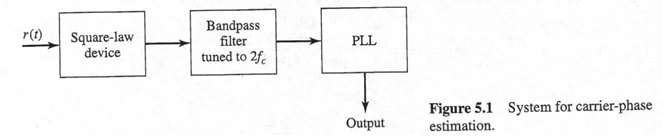
\includegraphics[scale = 1]{Implementazione del PLL nel demodulatore DSB-SC.png}
\end{figure} 

Gli elementi basilare di un PLL sono i seguenti: 

\begin{figure}[h]
    \centering
    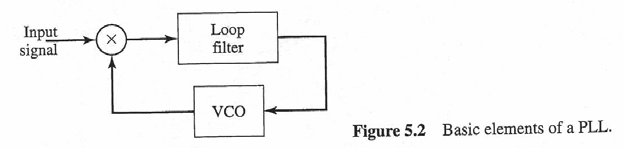
\includegraphics[scale = 1]{Elementi basilari di un PLL.png}
\end{figure} 

Quindi possiamo vedere l'esploso dello schema precedente (non quello del PLL), come: 

\begin{figure}[h]
    \centering
    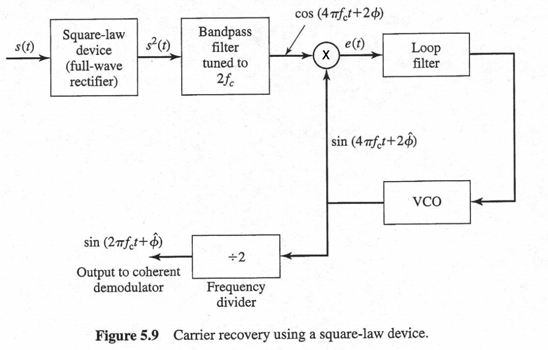
\includegraphics[scale = 1]{Recuperare la fase con un PLL e un demodulatore coerente DSB-SC.png}
\end{figure} 

\newpage 

Oppure possiamo utilizzare questo tipo di architettura: 

\begin{figure}[h]
    \centering
    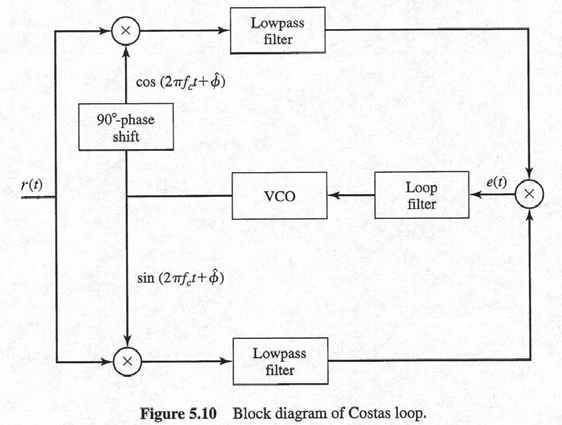
\includegraphics[scale = 0.8]{Sos.png}
\end{figure} 

\newpage 

\section{Effetto del rumore nelle modulazioni angolari}
\footnote{Slide del prof | Qualità nelle modulazioni analogiche | pag 7.2 \\  
Appunti di Damiano| pag 7.2 - 8.2\\
Slide | Qualità nelle modulazioni analogiche | pag 7.2 - 8.2 \\
Appunti | 2025-03-11 | pag 10 - 12 \\ 
Appunti | 2025-07-08 Ricevimento | pag 8.1
} 

Come rappresentato dai seguenti andamenti delle funzioni con modulazione angolare sovrapposto a del rumore: 

\begin{figure}[h]
    \centering
    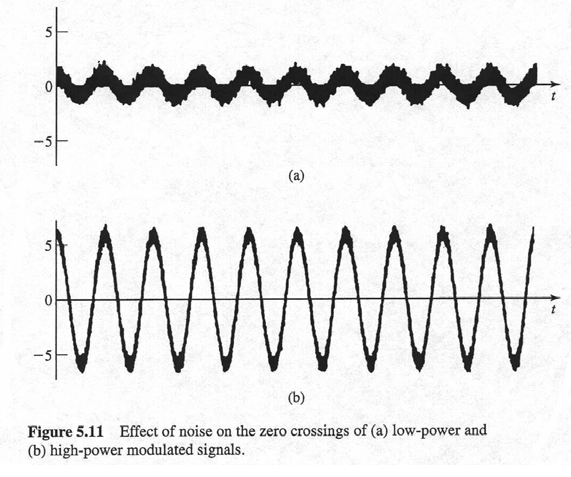
\includegraphics[scale = 1]{Rumore in una modulazione angolare.png}
\end{figure}

in particolare in alto un segnale a bassa potenza ed in basso un segnale ad alta potenza. \newline 

Il rumore cambia l'ampiezza, ma, nelle modulazioni angolari, l'informazione sta nei passaggi sullo zero. \newline 

Considerando dal punto di vista analitico il segnale modulato angolare u(t) con l'aggiunta del rumore n(t), 
abbiamo il segnale r(t) e distinguendo per la PM e la FM: 

{
    \Large 
    \begin{equation}
        \begin{split}
        r(t)
        &= 
        u(t)
        + 
        n(t)
        \\
        &= 
        A_c \cos(2 \pi f_c t + \phi (t))
        \\
        &= 
        \begin{cases}
            \begin{array}{ll}
            A_c \cos(2 \pi f_c t + k_p m(t)) + n(t) & \textbf{ PM} 
            \\
            \\
            A_c \cos \left( 2 \pi f_c t + 2 \pi k_f \int_{-\infty}^{t} m(\tau) d\tau \right)+ n(t) & \textbf{ FM}
            \end{array} 
        \end{cases}
        \end{split}
    \end{equation}
}

\newpage 

Utilizzando la rappresentazione dei fasori, 
possiamo visualizzare il contributo del rumore $\phi_n (t)$ sulla fase del segnale $\phi (t)$: 

\begin{figure}[h]
    \centering
    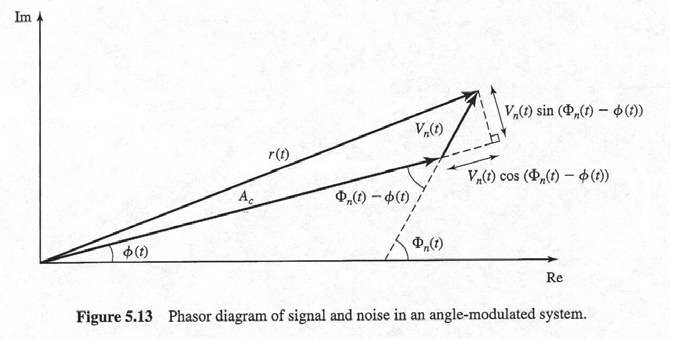
\includegraphics[scale = 1.2]{Rappresentazione sul piano dei fasori della modulazione angolare con il rumore.png}
\end{figure} 

Quindi il vettore r(t), senza rumore, dovrebbe coincidere con il vettore $A_c$, 
ma, a causa del vettore rumore $V_n (t)$, r(t) è uguale a: 

{
    \Large 
    \begin{equation}
        \overrightarrow{r(t)} = \overrightarrow{A_c} + \overrightarrow{V_n (t)}
    \end{equation}
}

quindi, il ricevitore, piuttosto che che visualizzare $\phi (t)$ visualizza $\phi (t) + \phi_n (t)$, cioè $\phi_t (t)$: 

{
    \Large 
    \begin{equation}
        \phi_t (t) = \phi (t) + \phi_n (t)
    \end{equation}
}

Facendo i calcoli (che sono omessi), la differenza tra quello che dovremmo ricevere in modulazione angolare $\phi (t)$ e quello che riceviamo realmente con il rumore, 
avremo $\gamma (t)$: 

{
    \Large 
    \begin{equation}
        \begin{split}
        \gamma (t) 
        &=
        \phi_n (t) - \phi (t) 
        \\
        &
        \arctan \left[\frac{V_n \sin(\phi_n (t) - \phi (t))}{A_c + V_n (t) \cos(\phi_n (t) - \phi (t))} \right] 
        \end{split} 
    \end{equation}
}

\begin{tcolorbox}
Non è necessario impararsi a memoria la formula  di $\gamma (t)$. \newline 

Basta sapere che il rumore con la sua fase $\phi_n (t)$ fa variare la fase in ricezione $\phi (t)$ e l'idea è quella di misurare la differenza tra le due fasi. \newline 

Idealmente vorremmo avere $\phi_n (t)$ nullo, ma ciò ,purtroppo, non capita
\end{tcolorbox}

\newpage 

\subsection{Demodulazione di segnali PM e FM}
\footnote{Slide del prof | Qualità nelle modulazioni analogiche | pag 9.1 - 11.2\\  
Appunti di Damiano| pag 9.1 - 11.2\\
Slide | Qualità nelle modulazioni analogiche | pag 9.1 - 12.2 \\
Appunti | 2025-03-11 | pag 13 \\
Appunti | 2025-07-08 Ricevimento | pag 4.2 - 7
} 

Considerando il caso in cui il rapporto segnale-rumore in ricezione elevato: 

{
    \Large 
    \begin{equation}
        \Pr{V_n (t) << A_c ^{2}} \approx 1
    \end{equation}
}

\begin{tcolorbox}
Essendo il rumore un processo stocastico, quindi probabilistico, 
formalmente non possiamo dire che si ha un rumore basso rispetto al segnale modulato. \newline 

Formalmente non possiamo scrivere: 

{
    \Large 
    \begin{equation}
        V_n (t) << A_c ^{2}
    \end{equation}
}

anche se di fatto si intende ciò con la formula di probabilità $\Pr{V_n (t) << A_c ^{2}} \approx 1$. 
\end{tcolorbox}

Considerando questo tipo di sistema: 

\begin{figure}[h]
    \centering
    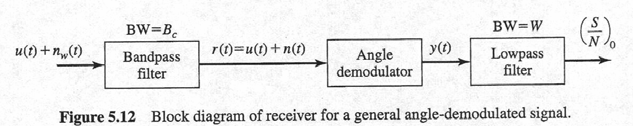
\includegraphics[scale = 1.4]{Diagramma di un demodulatore angolare.png}
\end{figure}

il segnale che esce dal demodulatore angolare y(t) è il seguente a seconda di PM e FM: 

{
    \Large 
    \begin{equation}
        y(t)
        = 
        \begin{cases}
            \begin{array}{ll}
            k_p m(t) + \frac{V_n (t)}{A_c} \sin(\phi_n (t) - \phi (t)) & \textbf{ PM} 
            \\
            \\
            k_f m(t) + \frac{1}{2 \pi} \frac{d}{dt} \left[ \frac{V_n (t)}{A_c} \sin(\phi_n (t) - \phi (t)) \right] & \textbf{ FM}
            \end{array} 
        \end{cases}
    \end{equation}
}

\newpage 

Di seguito la densità spettrale di rumore all'ingresso del filtro: 

\begin{figure}[h]
    \centering
    \includegraphics[scale = 0.7]{Densità spettrale di rumore all'ingresso del rumore.PNG}
\end{figure}

\begin{tcolorbox}
Questo grafico ci dimostra la densità spettrale del rumore in base alla modulazione utilizzata. \newline 

La figura in alto, quella indicata con (a), è la densità di rumore della PM, che rimane costante alle basse frequenze, cioè nell'intervallo tra -W e +W. \newline 

Oltre quell'intervallo, la densità di rumore diminuisce. \newline 

Questo significa che la PM è consigliata per le alte frequenze perché si avrà meno rumore al ricevitore. \newline 

Invece, notando la seconda figura in basso, quella indicato con (b), è la densità di rumore della FM, che ha un effetto parabolico e poi diventa quasi lineare oltre all'intervallo -W e +W. \newline 

Questo significa che la FM è consigliata per le basse frequenze perché si avrà meno rumore al ricevitore. \newline 

Per questo motivo, la FM è utilizzata nella radio commerciale (quella che ascolti tutti i giorni in macchina). \newline 

Nella realtà, grazie ai pregi e ai difetti delle due modulazioni angolari, si cercherà di fare una modulazione mista: una FM alle basse frequenze, una PM alle alte frequenze. \newline 

È possibile combinare le modulazioni angolari se abbiamo un sistema a banda molto larga; 
se la banda è molto stretta, quindi poco larga, si può utilizzare una tra le due. \newline 

Per questo ultimo motivo citato, ad esempio, la radio commerciale è a basse frequenze ed ha una banda molto stretta, quindi si utilizza solo la FM. 
\end{tcolorbox}

Quindi, dopo tutte queste considerazioni, possiamo esprimere le seguenti formule in caso di rapporto segnale-rumore all'ingresso del demodulatore sufficientemente elevato: 

{
    \Large 
    \begin{equation}
        \left( \frac{S}{N} \right)_{o}
        = 
        \begin{cases}
        \begin{array}{ll}
            \beta_p ^{2} P_{m_n} \left( \frac{S}{N} \right)_{b} & \textbf{ PM} 
            \\
            \\
            3 \beta_f ^{2} P_{m_n} \left( \frac{S}{N} \right)_{b} & \textbf{ FM}
        \end{array} 
        \end{cases}
    \end{equation}
}

\newpage 

Utilizzando l'effetto soglia, possiamo considerare questo grafico per confrontare il rapporto segnale-rumore 
scelto un $b_f$ rispetto all'SNR della modulazione DSB e SSB:

\begin{figure}[h]
    \centering
    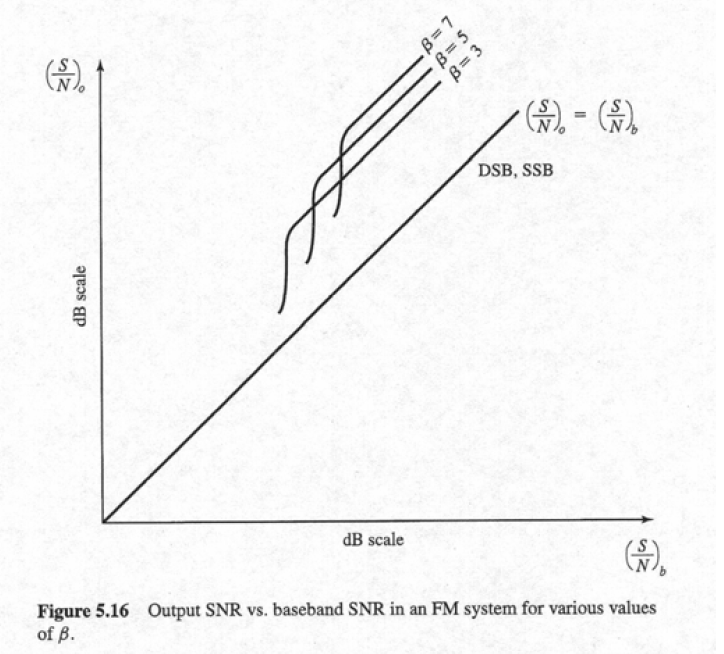
\includegraphics[scale = 0.7]{Confronto tra SNR in FM e quella in SSB.PNG}
\end{figure}

Utilizzando l'effetto soglia, in FM possiamo calcolarci il rapporto segnale-rumore: 

{
    \Large 
    \begin{equation}
        \left( \frac{S}{N}\right)_{b, th} = 20 (\beta + 1)
    \end{equation}
}

\begin{tcolorbox}
$\left( \frac{S}{N}\right)_{b, th}$ c'è il pedice th, perché dall'inglese si intende "threshold", cioè soglia. \newline 

Dato un certo valore di $\beta$, 
il valore $\left( \frac{S}{N}\right)_{b, th}$ è un valore approssimato della gobba della curva nella figura che si trova qui sopra. \newline 

Se abbiamo un $\left( \frac{S}{N}\right)_{b}$ minore della soglia, cioè $\left( \frac{S}{N}\right)_{b, th}$, non bisogna utilizzare la modulazione angolare 
perché il rapporto segnale-rumore in banda base sarà troppo piccolo, i.e. ci sarà più rumore rispetto al segnale utile e quest'ultimo non sarà ben reinterpretato dal ricevitore 
\end{tcolorbox}

Le caratteristiche del filtro per svolgere la pre-enfasi e la de-enfasi è la seguente: 

\begin{figure}[h]
    \centering
    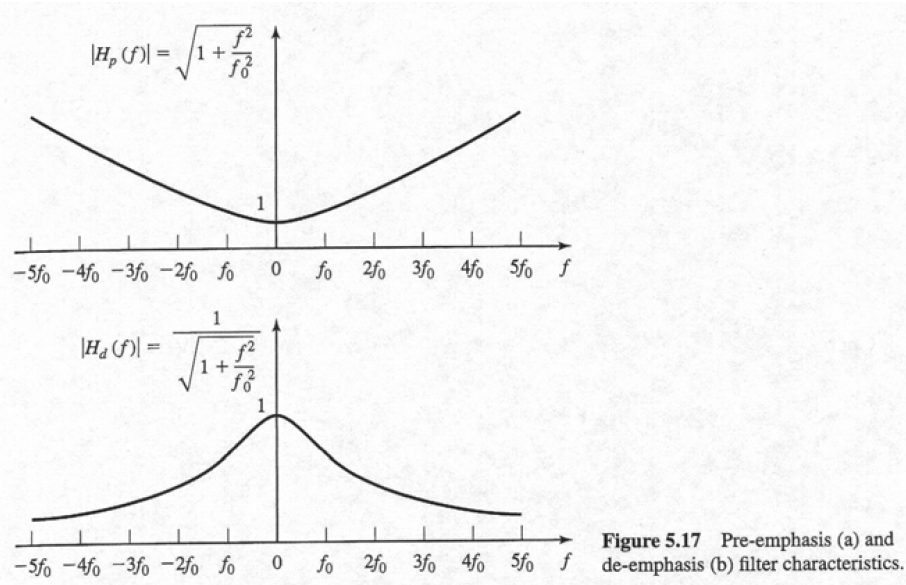
\includegraphics[scale = 0.7]{pre-enfasi e de-enfasi nella FM.PNG}
\end{figure}

\newpage 
